\documentclass[10pt,oneside,letterpaper]{article}
\usepackage[margin=1in]{geometry}

\usepackage{graphicx,color}
\usepackage{amsmath}
\usepackage{listings}
\usepackage[ruled,vlined]{algorithm2e}
\usepackage{listings}
\graphicspath{{./}{./figures/}}

\title{Merali13icra implementation}
\author{Vikas Dhiman}

\begin{document}
\maketitle

\section{Results}
Qualitative results are shown in Figure \ref{fig:results}. The map produced from MCMC Gibbs sampling has got some parts of the maps missing but it is relatively smoother than two-assumption algorithm. My MCMC Gibbs sampling implementation is slower than \cite{merali2013icra} implementation. While the authors claim that the complexity of the algorithm should be $O(maxSamples \times K \times N)$ where $K$ is the number of grid cells and $N$ is the number of observations. My implementation is $O(maxSamples \times K \times N \times F)$ where $F$ is the average number of cells traversed by a ray before finding an occupied cell. An additional complexity factor $O(F)$ is introduced by ray tracing for each observation to find the first occupied cell $f_{rn}$ in the path of the ray. On the other hand \cite{merali2013icra} somehow compute $p(z_n|f_{rn})$ in $O(1)$ time-complexity.

I believe the smoothness of results in MCMC Gibbs sampling method is not because we drop inter-cell independence assumption. Instead it is because we use Gaussian forward sensor model in case of MCMC Gibbs sampling while a step function for Two-assumption method.

\begin{figure}
  
\includegraphics[width=0.3\textwidth]{figures/gt-final.png}
  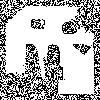
\includegraphics[width=0.3\textwidth]{figures/mcmc_100x100.png}
  
\includegraphics[width=0.3\textwidth]{figures/two-assumption_100x100.png}
  \caption{From left to right: 1) Observed ground truth (resolution: 500x500) 2) Map generated by MCMC Gibbs sampling as described in \cite{merali2013icra} with  $20 \times 10^4$ samples(resolution:100x100) 3) Map generated by two-assumption method as described in \cite{merali2013icra} (resolution:500x500) }
  \label{fig:results}
\end{figure}
\begin{figure}
  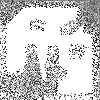
\includegraphics[width=0.3\textwidth]{figures/Metropolis_Marginals_20k_iter.png}
  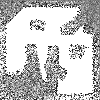
\includegraphics[width=0.3\textwidth]{figures/Metropolis_Marginals_40k_iter.png}
  
\includegraphics[width=0.3\textwidth]{figures/metropolis_100x100.png}
  \caption{From left to right: Marginals computed by metropolis hastings algorithm with 1) $2 \times 10^4$ samples (resolution:100x100) 2) with $4 \times 10^4$ samples and 3) with $10 \times 10^4$ samples }
  \label{fig:metropolis-results}
\end{figure}

\section{Input Data}
I have used \emph{Player 3.0.2} and \emph{Stage 3.2.2} \cite{gerkey2003player} for simulating input data. The configuration file and map used are in the repository : worlds/simple.cfg.

\begin{figure}
  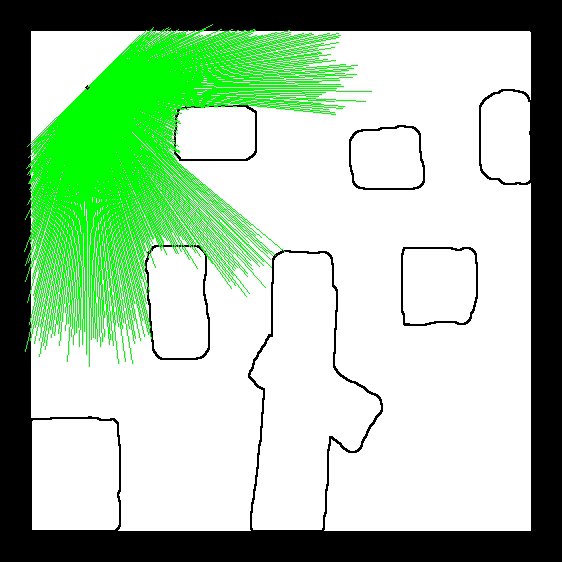
\includegraphics[width=0.3\textwidth]{figures/input-start.png}
  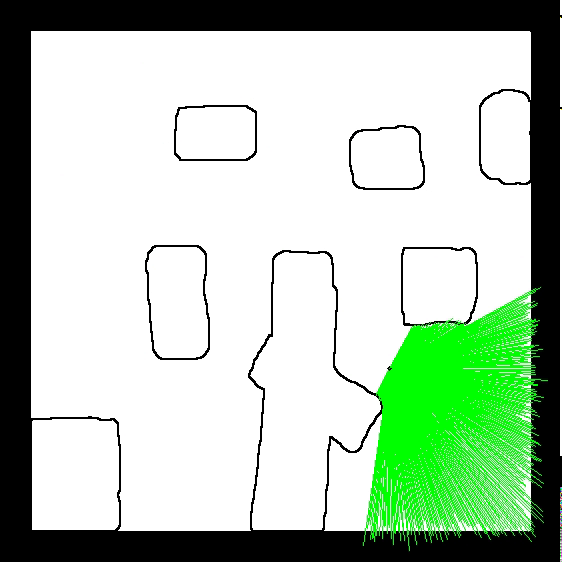
\includegraphics[width=0.3\textwidth]{figures/input-mid.png}
  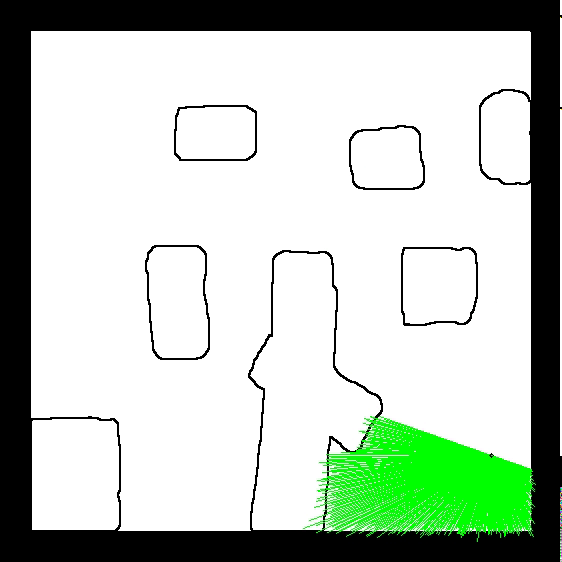
\includegraphics[width=0.3\textwidth]{figures/input-last.png}
  \caption{Random snapshots of Robot moving through given map. The laser data is perturbed by Gaussian noise that increases linearly with distance. The robot does not observes all regions of the map, so the observed ground truth is a subset of ground truth map. Observed ground truth is shown in Figure \ref{fig:results}}
  \label{fig:input}
\end{figure}
% Launch player:
% \lstset{language=Bash}
% \begin{lstlisting}
%   player worlds/simple.cfg
% \end{lstlisting}
% 
% Launch capture script:
% \begin{lstlisting}
%   cpp/build/bin/captureplayerdata
% \end{lstlisting}

\section{MCMC Gibbs sampling }

\subsection{Forward sensor model}
The probability $p(z_n|x_n, m^r)$ represents the forward sensor model which is computed by assuming that the pose is exactly known and using ray tracing to find the first occupied cell, $f_{r,n}$ that the laser hits for a given map $m_r$ and pose $x_n$. Let the distance between position of laser and the first occupied cell it hits in $m^r$ be $z^r_n$. Assuming Gaussian noise that whose variance increases linearly with distance ($\sigma' = \sigma z^r_n$),  the probability of observation $z_n$ given map $m^r$ and pose $x_n$ is given by: 
\begin{align}
  p(z_n|x_n, m^r) &= N(z_n|z^r_n, \sigma z^r_n)
\end{align}
where $N(x|\mu, \sigma)$ represents Gaussian at $x$ with mean $\mu$ and variance $\sigma$. We choose the variance to be $\sigma z^r_n$ ($\sigma = 0.05$ for our experiments). The scale factor of Gaussian is ignored and probability is computed in Log domain:
\begin{align}
  \log p (z_n|x_n, m^r) &= \frac{(z_n - z^r_n)^2}{(\sigma z^r_n)^2}
  \label{eq:fwdmodel}
\end{align}
Equation \eqref{eq:fwdmodel} is implemented in function \emph{log\_odds\_single\_observation\_given\_map\_and\_pose} in file 
\emph{cpp/src/forward\_sensor\_model.cpp}. Ray tracing for the computation of $z^r_n$ given map $m^r$ and pose $x_n$ is implemented in method \emph{OccupancyGrid2D::ray\_trace}. Both $\log p(z_n|x_n, m_{\neg k}, m_k = 1)$ and $\log p(z_n|x_n, m_{\neg k}, m_k = 0)$ can be computed using \eqref{eq:fwdmodel}.

\subsection{Prior}
The prior $p(m_k = 1 | m_{\neg k})$ is assumed to be constant and unbiased i.e $0.5$. Equations (3) from \cite{merali2013icra} are implemented in function \emph{probabability\_occupied\_to\_free}

\subsection{Gibbs sampling}
Algorithm 1 from \cite{merali2013icra} is implemented as function \emph{inference\_gibbs\_sampling} in \emph{cpp/src/inference\_gibbs\_sampling.cpp}

\section{Two-assumption method }
This method is described in Section II of \cite{merali2013icra}. I have implemented this method in \emph{cpp/src/two\_assumption\_alg.cpp}. Prior probability is assumed to be unbiased and with log likelihood as 0. While the ray traverses through cell $\kappa$ with observation given to be $z_n$ the map is updated using the following step function as mentioned in \cite{merali2013icra}:
\begin{align}
  l(m_{\kappa}|z_n, x_n) &= \begin{cases}
         l_{\text{free}} & \text{if $\kappa < z_n$}\\
          l_{\text{occ}} & \text{if $\kappa = z_n$}\\
                       0 & \text{otherwise}
  \end{cases}
\end{align}

\section{Metropolis Hastings}

I have got the results for Metropolis Samplings without using the heatmap
(Figure \ref{fig:metropolis-results}). Metropolis sampling converges better
than Gibbs sampling because we don't waste time in exploring low probability
(free) areas. Moreover, the present results are a result of biased random walk.
Brian's code chose a cell by uniformly sampling over the entire map. In an
attempt to keep samples to near high occupancy regions, I modified the sampling
strategy to use Gaussian in case of acceptance, and uniform sampling in case of
rejection. In case of acceptance, I use the previously chosen cell as the mean
and a heuristic variance (5\% of grid height/width) for finding the next cell
to flip. This strategy works with the assumption that areas of high probability
are clustered together in the occupancy grid (in the two dimensional space
apart from the 100x100 dimensional space that is being explored by metropolis
hastings algorithm.

\section{Speed up}

I used a caching strategy to speed up energy computation. For the first time, I
compute the total energy due to all factors (laser observations). For
subsequent iterations, I recompute only those factors that are related the cell
whose occupancy has changed. Though this strategy is generic and can be
implemented without change of interface, it uses a lot of memory to maintain
energy corresponding to each factor ($2.6 \times 10^5$ factors for my data
set). Moreover, it has to check of the changed occupancy by looping over all
the cells in the map. Currently $4 \times 10^4$ samples of metropolis hastings
with $2.6 \times 10^5$ laser observations (number of laser scans $\times$
lasers readings per scans) takes around 82 seconds. As per \emph{perf} tool
profiling results, 60\% of the time is spent in caching.

Another option to speed up is to just calculate the delta i.e. $Ex - Ex'$, which will require a change of interface i.e. to change the meaning of what \emph{operator()} does for a factor graph according to gtsam conventions. However, speed gain may not be more than 5\%.

\section{Belief Propagation}
I have got results from Belief Propagation algorithm. 
Although the general version of sum product algorithm is almost impossible to work with because of large neighbourhood size. For example, if a laser passes through 20 cells that means that the laster factor has 20 neighbours in the factor graph and hence $2^{20}$ terms to sum upon. The expression for computing sum product marginal is given by
\begin{align}
  \mu_{f \rightarrow x_i}(x_i) &= \sum_{\sim\{x_i\}} f(N(f)) \prod_{y \in N(f) \setminus \{x_i\}} \mu_{f \rightarrow y}(y)
\end{align}
where $\sum_{\sim\{x_i\}}$ represents marginalization i.e. summation over all possible assignments of $N(f)$ while keeping $x_i$ fixed.

However, the sum product term can be simplified in case of different functions including the piecewise constant function that we have. After simplification the belief computation over a factor becomes linear in number of neighbors as compared to exponential in the general case.
\begin{align}
  f(N(f)) &= \begin{cases}
       w_0 & \text{ if } N(f) = \mathbf{x_{0}}\\
       w_1 & \text{ if } N(f) = \mathbf{x_{1}}\\
       w_2 & \text{ otherwise}
  \end{cases}
\end{align}
\begin{align}
  \mu_{f \rightarrow x_i}(x_i) &= 
    w_0 \prod_{x \in N(f) \setminus \{x_i\}} \mu_{f \rightarrow x}(x_{0})  +
    w_1 \prod_{x \in N(f) \setminus \{x_i\}} \mu_{f \rightarrow x}(x_{1}) +\\
    & w_2 \left(1 - \prod_{x \in N(f) \setminus \{x_i\}} \mu_{f \rightarrow x}(x_{0})
    - \prod_{x \in N(f) \setminus \{x_i\}} \mu_{f \rightarrow x}(x_{1})\right) 
\end{align}

Fig. \ref{fig:bpresults} shows belief propagation results. In each iteration a random edge was chosen and belief updated by belief propagation algorithm. 4 million iterations were completed in about 90 seconds.
\begin{figure}
  
\includegraphics[width=0.3\textwidth]{bpresults_100x100_50.png}
  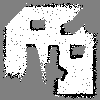
\includegraphics[width=0.3\textwidth]{bpresults_100x100_200.png}
  
\includegraphics[width=0.3\textwidth]{beliefpropagation_results_100x100.png}
  \caption{Belief propagation results after a) 0.5 million iterations b) 2 million iterations and c) 4 million iterations}
  \label{fig:bpresults}
\end{figure}

We have not yet introduced smoothness factors, which means that the only factors are laser factors and that causes belief propagation to updated beliefs of only relevant areas in the occupancy grid where we have some kind of information available.

\section{Dual decomposition}
Dual decomposition \cite{sontag2011introduction} works by allowing factors to optimize their copy of variable nodes and later resolve the disagreements by passing messages.  Dual decomposition at 100x100 resolution takes about 7 seconds per iteration. Results are shown in Fig \ref{fig:dualdecomposition}. The effect of dual decomposition iterations is not evident at a 100x100 resolution. So I also have results at 500x500 resolution in Fig \ref{fig:dualdecomposition500x500}. Initially the edges are washed out because of noisy observations. After few iterations the edges emerge out. At 500x500 resolution each iteration of dual decomposition takes around 27 seconds. Though the number of Variable disagreement resolved throughout entire routine is pretty low. For 500x500 resolution, the 50925 variables disagree among their respective copies, by the end of 100 iterations the number is reduced to 50007 which is a reduction by 1.8\% over 100 iterations. 
\subsection{Advantages of dual decomposition}
\begin{itemize}
  \item When most of the factors agree with each other, we should use dual decomposition as it starts with a reasonable solution in such a case by postponing the disagreements.
\end{itemize}
\subsection{Disadvantages of dual decomposition (Subgradient method)}
\begin{itemize}
  \item Since it solves to get the minimum energy assignment, we do not get marginals for each variable but instead a best assignment. For disagreeing nodes, this assignment can be quite arbitrary.
  \item Convergence of the algorithm can be quite slow and depends on the step size in subgradient descent algorithm.
  \item It is tough to figure out, when the algorithm has converged as equally disagreeing nodes may never agree on a solution, hence quite likely the number of disagreeing nodes will never reduce to zero.
\end{itemize}
\begin{figure}
  
\includegraphics[width=0.25\textwidth]{dualdecomposition0_100x100.png}%
  
\includegraphics[width=0.25\textwidth]{dualdecomposition10_100x100.png}%
  
\includegraphics[width=0.25\textwidth]{dualdecomposition20_100x100.png}%
  
\includegraphics[width=0.25\textwidth]{dualdecomposition30_100x100.png}
  \caption{Dual decomposition results at 100x100 resolution after a) 1 iteration b) 10 iterations c) 20 iterations and d) 30 iterations}
  \label{fig:dualdecomposition}
\end{figure}

\begin{figure}
  
\includegraphics[width=0.25\textwidth]{dualdecomposition0_200x200.png}%
  
\includegraphics[width=0.25\textwidth]{dualdecomposition33_200x200.png}%
  
\includegraphics[width=0.25\textwidth]{dualdecomposition66_200x200.png}%
  
\includegraphics[width=0.25\textwidth]{dualdecomposition98_200x200.png}
  \caption{Dual decomposition results at 200x200 after a) 1 iteration b) 34 iterations c) 67 iterations and d) 100 iterations}
  \label{fig:dualdecomposition200x200}
\end{figure}

\begin{figure}
  
\includegraphics[width=0.25\textwidth]{dualdecomposition0_500x500.png}%
  
\includegraphics[width=0.25\textwidth]{dualdecomposition33_500x500.png}%
  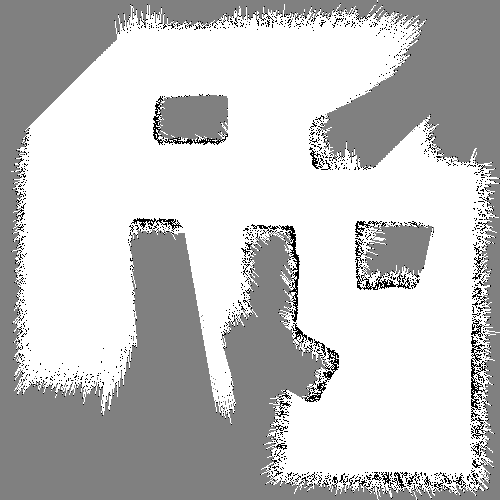
\includegraphics[width=0.25\textwidth]{dualdecomposition66_500x500.png}%
  
\includegraphics[width=0.25\textwidth]{dualdecomposition99_500x500.png}
  \caption{Dual decomposition results at 500x500 after a) 1 iteration b) 34 iterations c) 67 iterations and d) 100 iterations}
  \label{fig:dualdecomposition500x500}
\end{figure}

\lstset{language=bash}
\begin{lstlisting}
vikasdhi@redpanda:~/wrk/OccupancyGrid$ bin/dualdecomposition 18 18 .09
Factor disagreement count:554496
Total energy:554496
i=0 clicks taken: 17.68
Variable disagreement count:14563
Factor disagreement count:277248
Total energy:1.85523e+07
i=1 clicks taken: 11.67
Variable disagreement count:14557
...
... After 100 iterations
...
Factor disagreement count:277248
Total energy:8.9673e+07
i=99 clicks taken: 11.5
Variable disagreement count:14483
\end{lstlisting}

\begin{lstlisting}
vikasdhi@redpanda:~/wrk/OccupancyGrid$ bin/dualdecomposition 18 18 .036
Factor disagreement count:554496
Total energy:554496
 clicks taken: 42.88
Variable disagreement count:50925
Factor disagreement count:277248
Total energy:2.25915e+07
 clicks taken: 25.32
Variable disagreement count:50911
...
... After 100 iterations
...
Factor disagreement count:277248
Total energy:1.07315e+08
 clicks taken: 25.53
Variable disagreement count:50007
\end{lstlisting}

\section{Convergence comparison}
Please see Fig~\ref{fig:convergence-comparison}, Fig~\ref{fig:convergence-comparison-visuals} and Table~\ref{tab:convergencetime}.
\begin{figure}
  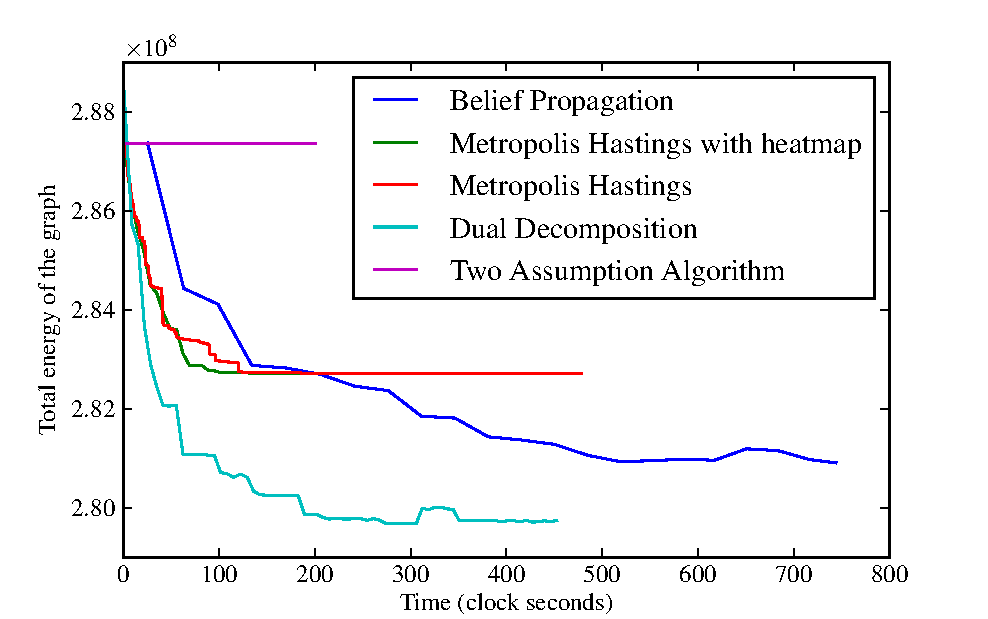
\includegraphics[width=\textwidth]{figures/relativeconvergence.pdf}%
  \caption{Comparison of convergence of different algorithms on occupancy grid graph. While sampling methods like Metropolis hastings converge quickly they stay far from optimum energy. On the other hand modern minimization algorithms reach closer to an optimum value.}
  \label{fig:convergence-comparison}
\end{figure}
\begin{figure}
  
\includegraphics[width=0.2\textwidth]{figures/bpresults_100x100_200sec.png}%
  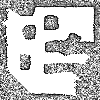
\includegraphics[width=0.2\textwidth]{figures/SICKDDMCMC200sec_100x100.png}%
  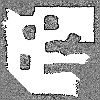
\includegraphics[width=0.2\textwidth]{figures/SICKSlowMetropolis200sec_100x100.png}%
  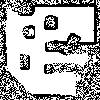
\includegraphics[width=0.2\textwidth]{figures/dualdecomposition200sec_100x100.png}%
  
\includegraphics[width=0.2\textwidth]{figures/TwoAssumptionAlgo200sec_100x100.png}%
  \caption{Qualitative results at the end of 200sec for each algorithm (from left to right) a) Belief Propagation b) Metropolis Hastings with heat map c) Metropolis Hastings without heat map d) Dual decomposition e) Two assumption algorithm}
  \label{fig:convergence-comparison-visuals}
\end{figure}

\begin{table}
  \begin{tabular}{|l|r|r|r|}
    \hline
                                     & Time taken (sec) & Iterations \\
    \hline
    Belief Propagation               & 321.16           & 1.03213e+07\\
    Metropolis hastings with heatmap & 136.87           & 50000\\
                  Metropolis hastings& 249.20           & 150000\\
    Dual Decomposition               & 353.85           & 70\\
    Two assumption algorithm         & 2.27             & 1\\
    \hline
  \end{tabular}
  \caption{Table showing the number of iterations and time taken for the algorithm}
  \label{tab:convergencetime}
\end{table}


%\IEEEtriggeratref{5} % manually align last two columns
\bibliographystyle{plain}

\bibliography{/home/vikasdhi/wrk/biblib/bibdb}
\end{document}
